\section{Durchführung und Aufbau}
\label{sec:Durchführung}
Anhand der Messaperatur aus Abbildung \ref{fig:Mess} sollen das Torsionsmodul bestimmt werden.
\begin{figure}
  \centering
  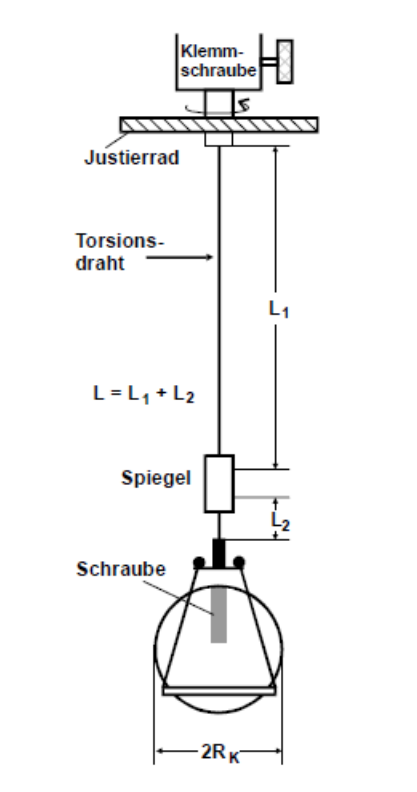
\includegraphics[height=10cm]{picture/Messapperatur.png}
  \caption{Apparatur zur Bestimmung des Torsionsmodul}
  \label{fig:Mess}
\end{figure}
\subsection{Daten der Messaperatur}
Dafür wird zunächst di Länge $L_1$ sowie $L_2$ je drei mal vermessen und der Durchmesser an verschiedenen Stellen insgesamt fünf mal. Die weiteren Daten mit den entsprechenden Messunsicherheiten werden dem Versuchsaufbau entnommen.
\subsection{Schwingungsdauer des Torsionsmodul ohne Magnetisches Moment}
Es ist drauf zu achten das die Dipolachse des Magneten senkecht zum Erdmagnetfeld steht. Anschleißend wird der Draht am Justierrad um kleine Winkel ausgelengt so das der Lichtstrahl welcher von der Lichtquelle den Spiegel trifft aufgrund der Trosion um den Lichtdetektor pendelt (siehe Abbildung \ref{fig:Aufbau}). Um unerwünschte Pendelbewegung zu verhindern wird mittels einem Dämpfer versucht die Pendelbewegungen zu minimieren. Die Taktung des Lichtdetektors soll so geschaltet werden, dass bei dem ersten durchlauf jeweils das Zählwerk startet, beim dritten Stopt und beim vierten mal das Zählwerk zurückgestellt wird. Es werden 10 Perioden gemessen und die Werte notiert.
\begin{figure}
  \centering
  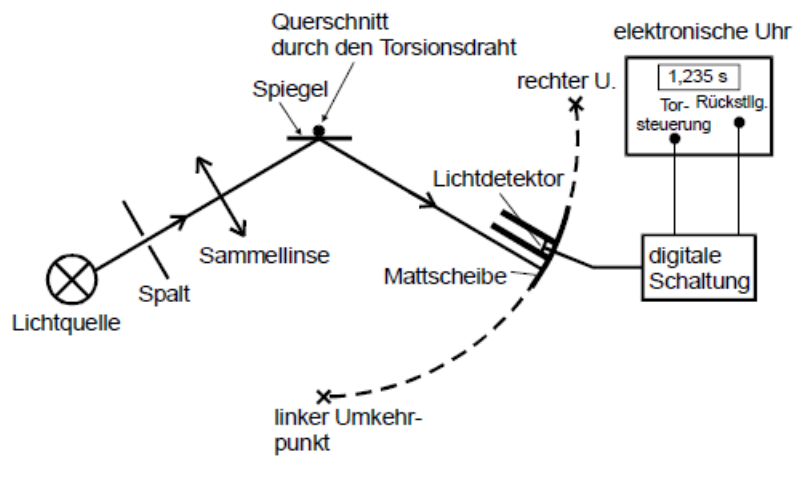
\includegraphics[height=7cm]{picture/Aufbau.png}
  \caption{Aufbau der Messaperatur.}
  \label{fig:Aufbau}
\end{figure}
\subsection{Messung des Erdmagnetfeldes}
Die Dipolachse des Magneten wird entsprechend der Feldlinien des Erdmagnetfeldes parallel gelegt und die Schwingungsdauer erneut 10 mal bestimmt. Anhand dessen lässt sich die Stärke des Erdmagnetfeldes ableiten.
\subsection{Messung des Erdmagnetfeldes}
Um das magnetische Moment des Stabmagneten zu messen wird der Aufbau Abbildung \ref{fig:Aufbau2} modifiziert. 
\begin{figure}
  \centering
  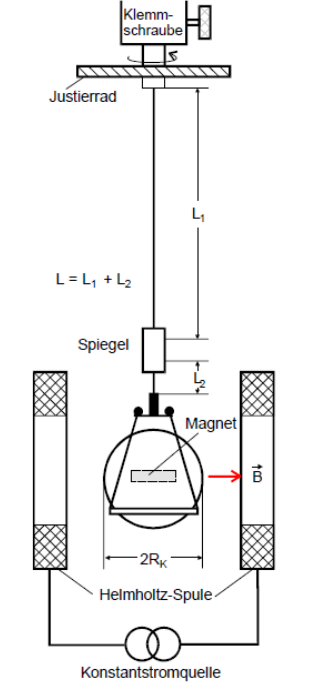
\includegraphics[height=8cm]{picture/Aufbau2.png}
  \caption{Messaperatur zur Vermmesung des Dipolmoments.}
  \label{fig:Aufbau2}
\end{figure}
Es werden die Schwingungsdauern von fünf Perioden entnommen bei fünf verschiedenen Feldstärken  der Helmholzspulen. Dabei ist darauf zu achten das die Dipolachse möglichst parallel zu dem Magnetfeld der Helmholtzspulen ausgerichtet ist. 
